\section{Results}
\label{s:results}

    The diffraction patterns for ZnO:Ga, ZnO:Ga@SiO$_{2}$ and {\znoo} are shown in \cref{fig:xrdp_znO}. They are all in agreement with that of ZnO:Ga standard (card No. 01-073-1368) from ICDD PDF-2 database. Prepared materials correspond to  hexagonal crystal structure of wurtzite. The absence of additional peaks in diffraction patterns excludes the presence of any other crystalline phase. Narrow diffraction peaks indicates larger crystallites. Electron microscopy confirmed larger crystallites, the size of nanocomposite was at the limit of measurability thus images are a little bit blurred. Scans from scanning electron microscopy are shown in the \cref{fig:sem_znoga,fig:sem_zgs,fig:sem_zgsp}.\\
    
    \begin{figure}
        \centering
        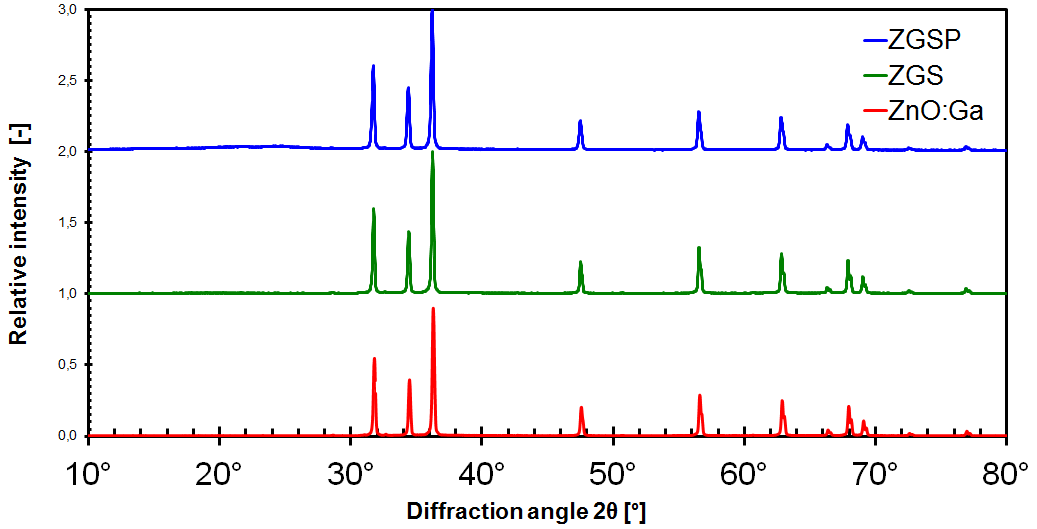
\includegraphics[width=0.8\textwidth]{pictures/xrd_januar_18.PNG}
        \caption{XRDP diffraction patterns of synthesized nanoparticles for ZnO:Ga, ZnO:Ga@SiO$_{2}$ (ZGS) and {\znoo} (ZGSP). Data for ZnO:Ga@SiO$_{2}$ and {\znoo} are vertically shifted for better visualization.}
        \label{fig:xrdp_znO}
    \end{figure}
    
\begin{figure}
    \centering
        \hspace*{\fill}%
    \begin{minipage}{.3\textwidth}
        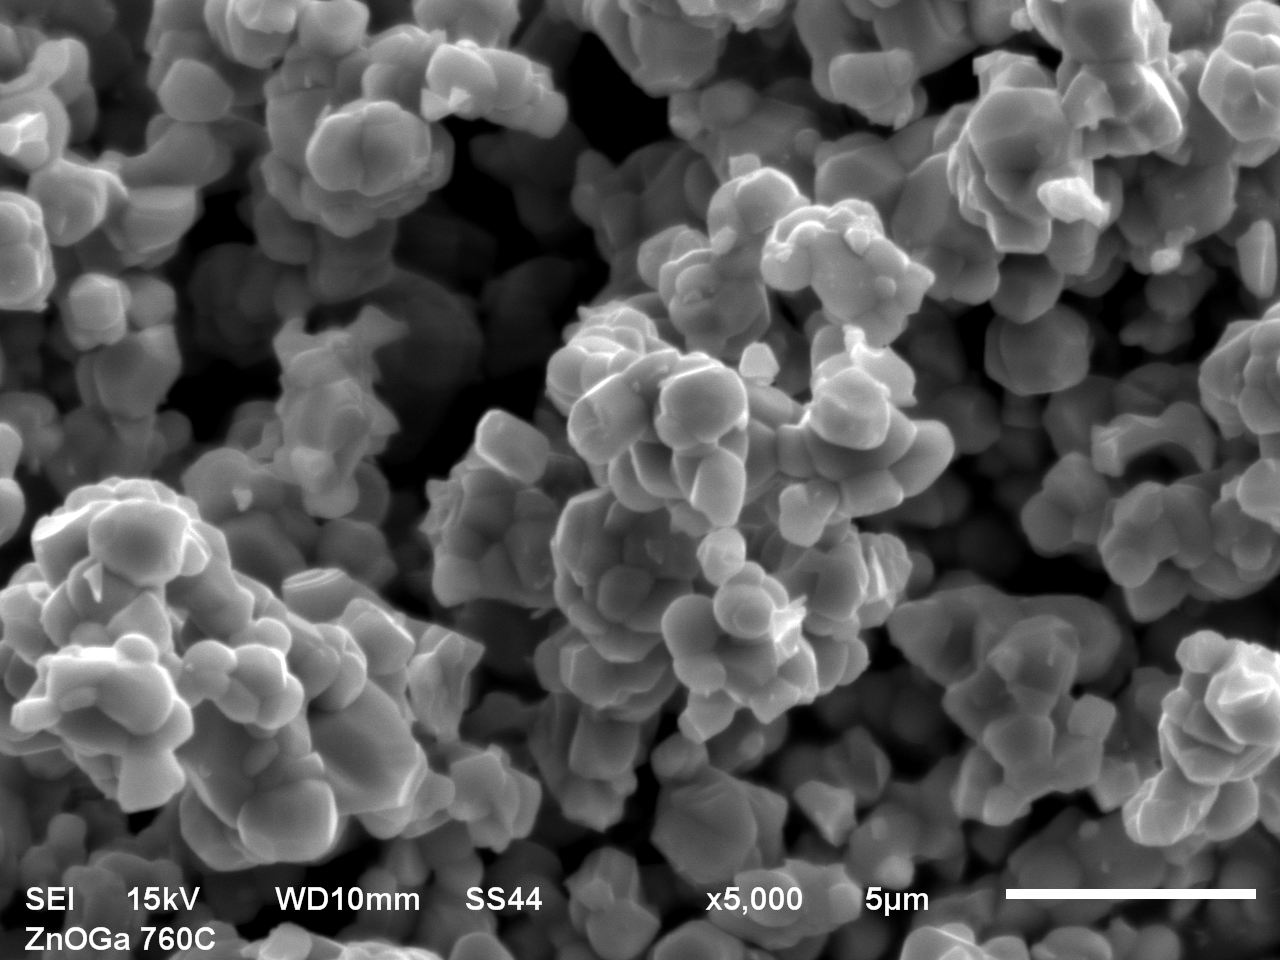
\includegraphics[width=\textwidth]{pictures/sem_ZnOGa_5_mikro.png}
        \caption{SEM scan of ZnO:Ga.}
        \label{fig:sem_znoga}
    \end{minipage}
      \hspace{\fill}%
    \begin{minipage}{.3\textwidth}
        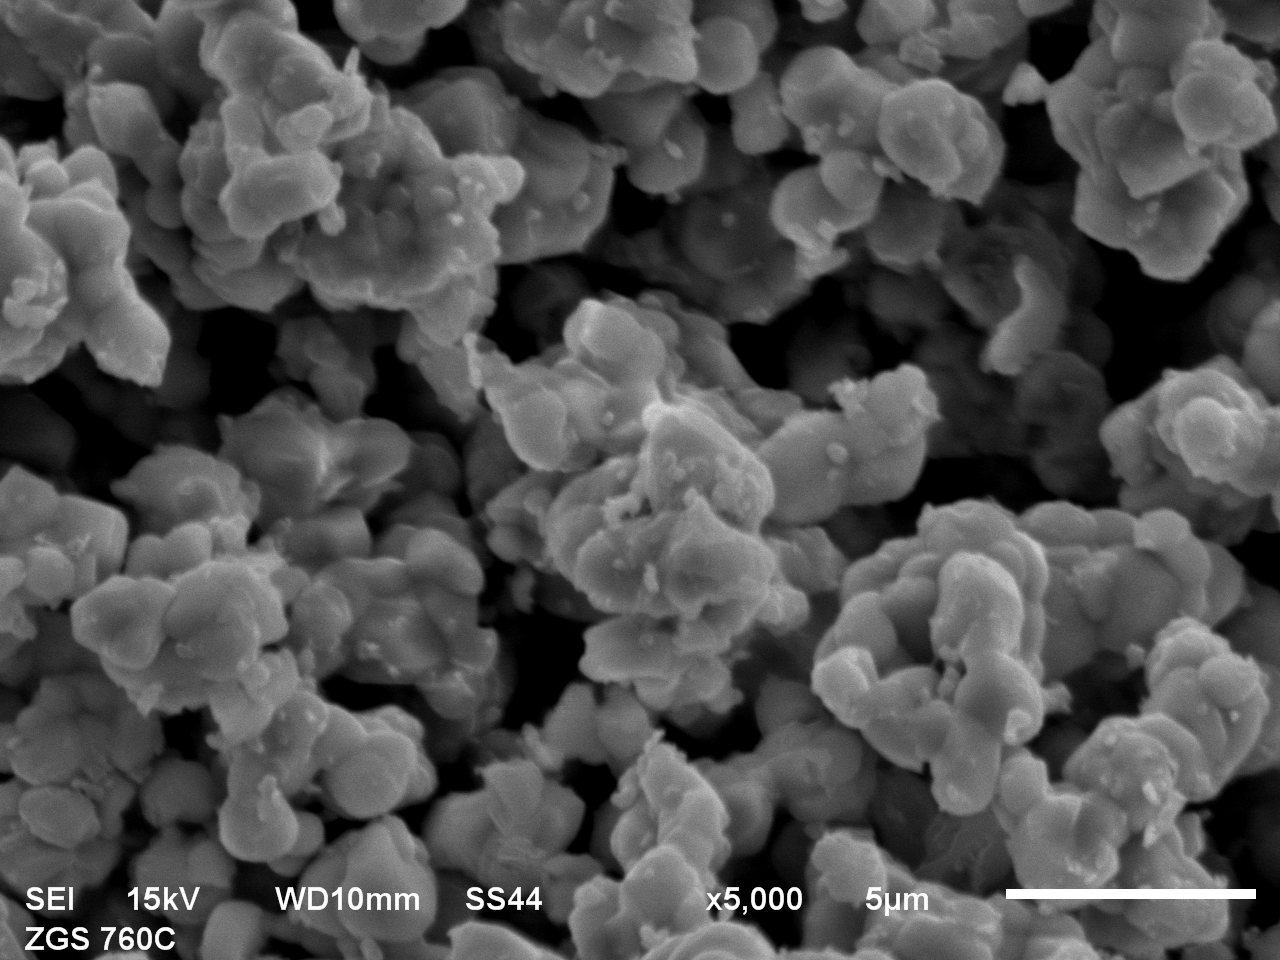
\includegraphics[width=\textwidth]{pictures/sem_ZGS_5_mikro.png}
        \caption{SEM scan of ZnO:Ga@SiO$_{2}$.}
        \label{fig:sem_zgs}
    \end{minipage}
        \hspace*{\fill}%
    \begin{minipage}{.3\textwidth}
        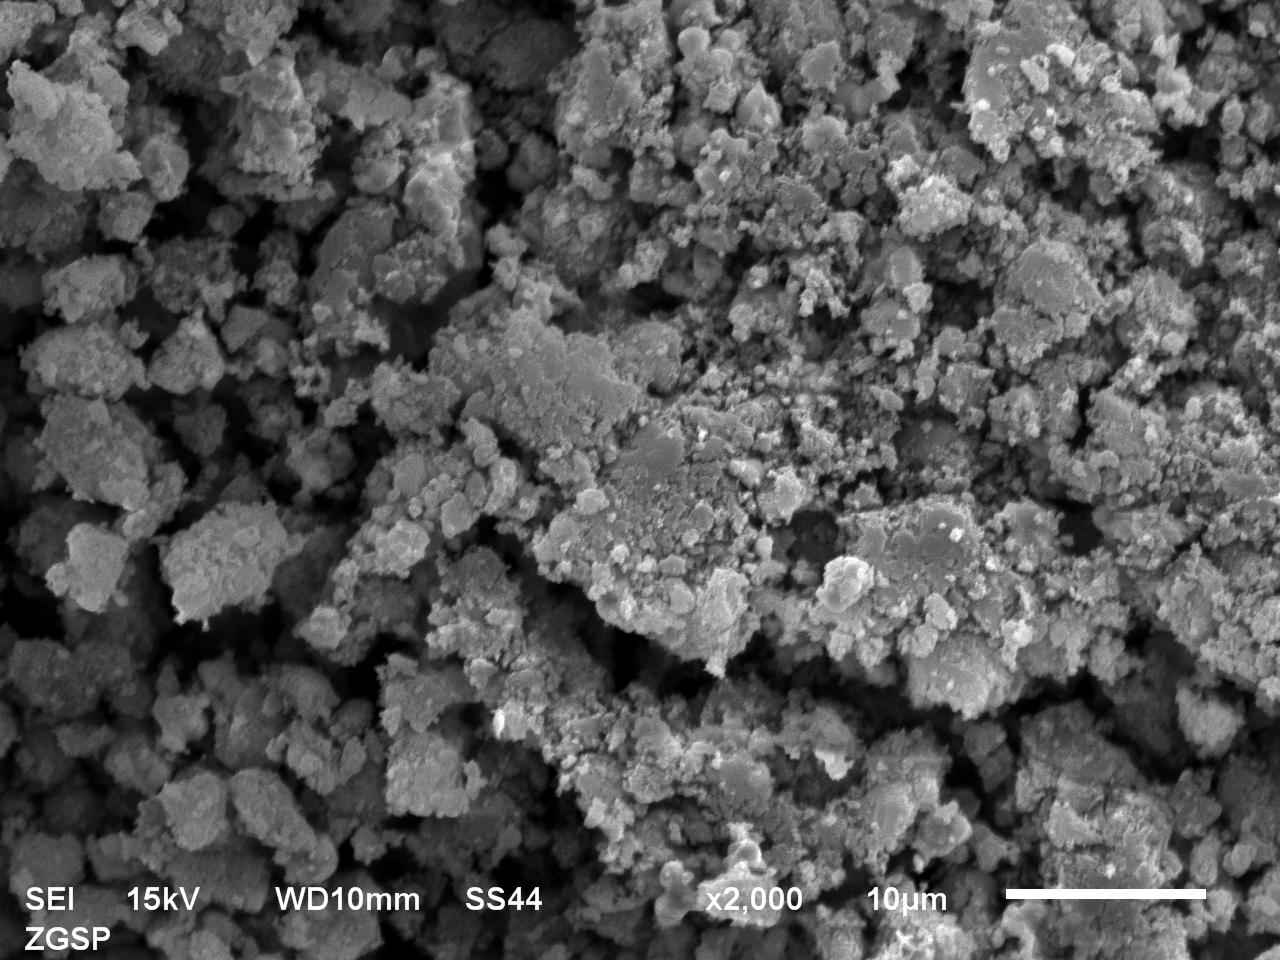
\includegraphics[width=\textwidth]{pictures/sem_ZGSP_10_mikro.png}
        \caption{SEM scan of {\znoo}.}
        \label{fig:sem_zgsp}
    \end{minipage}
        \hspace*{\fill}%
\end{figure}

    The \cref{fig:znoga_januar_rt_pl} shows RL and PL emission spectra of Zno:Ga and {\znoo}. The diffrence in the intensities of luminescence at \numprint[nm]{590} and at \numprint[nm]{650} is observed. This difference is caused by conjugation of PPIX in nanocomposite. It is not clear why PL emission spectrum of {\znoo} do not show any emission peak of ZnO:Ga at \numprint[nm]{390}. Non-radiation energy transfer probably takes place between ZnO:Ga and PPIX since PPIX peaks at \numprint[nm]{590} and \numprint[nm]{650} are observed and emission of ZnO:Ga at \numprint[nm]{390} is not observed.\\
    
    \begin{figure}[h]
        \centering
        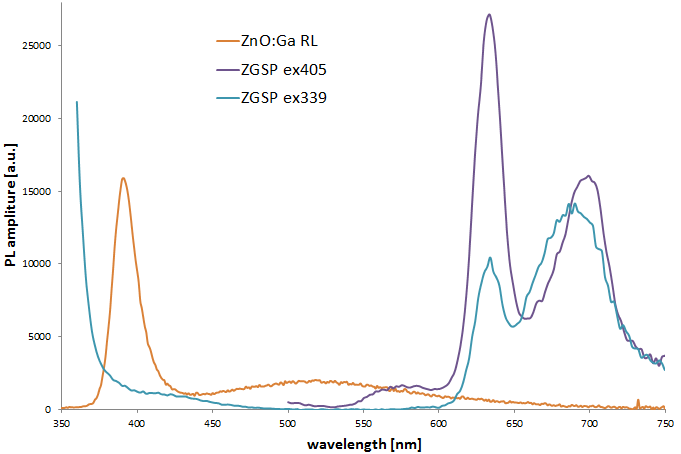
\includegraphics[width=0.6\textwidth]{pictures/znoga_januar_rt_pl.PNG}
        \caption{RL and PL emission spectra of ZnO:Ga and ZnO:Ga@SiO$_{2}$-PPIX (ZGSP) under \numprint[nm]{339} and \numprint[nm]{405} excitation.}
        \label{fig:znoga_januar_rt_pl}
    \end{figure}
    
    
    In addition PL decay curves under \numprint[nm]{339} and \numprint[nm]{389} excitation were measured, they are shown in the \cref{fig:zgs_januar_340ex_390em,fig:zgsp_januar_340ex_390em,fig:zgsp_januar_340ex_630em,fig:zgsp_januar_389ex_630em}. 
    From previous characterization it is obvious that decay time of ZnO:Ga is about \numprint[ns]{0.5} and decay time of PPIX is about \numprint[ns]{3}. 
    The \cref{fig:zgsp_januar_340ex_390em} shows decay time \numprint[ns]{2.4} which belongs to PPIX. 
    In the \cref{fig:zgsp_januar_340ex_630em} and \cref{fig:zgsp_januar_389ex_630em}, decay time of ZnO:Ga@SiO2-PPIX is about \numprint[ns]{12}. 
    This decay times could belong to free PPIX in dilute solution. 
    In comparison with other experiments, it is obvious that the decay times belong to PPIX and not to SiO$_{2}$ shell.
    
    Within the measurements luminescence was really low that could cause unmeasurable conditions or refer to the preparation of the material was not realized correct.\\
    
    \begin{figure}
        \centering
        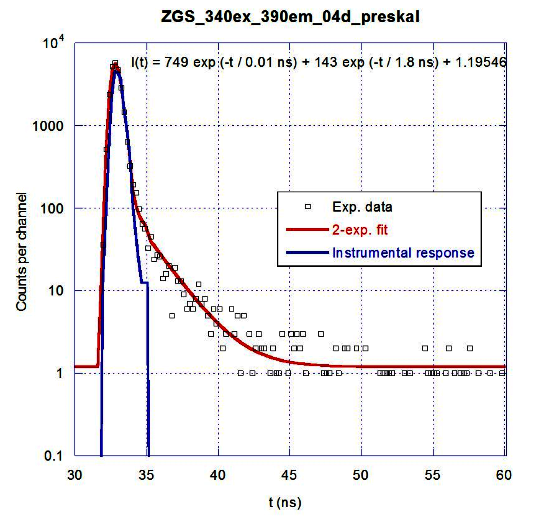
\includegraphics[width=0.6\textwidth]{pictures/zgs_januar_340ex_390em.PNG}
        \caption{PL decay of ZnO:Ga@SiO2 in EtOH under \numprint[nm]{339} excitation, emission \numprint[nm]{390}.}
        \label{fig:zgs_januar_340ex_390em}
    \end{figure}
    
    \begin{figure}
        \centering
        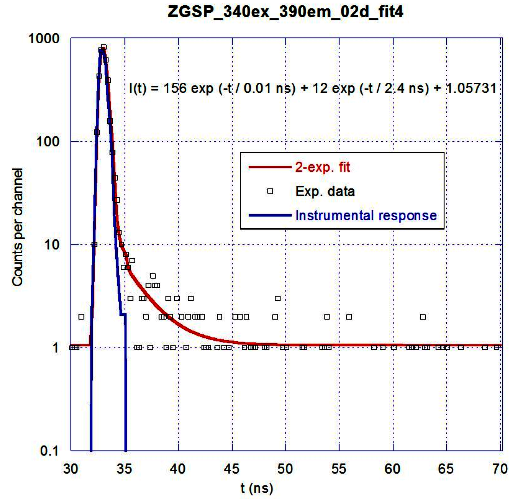
\includegraphics[width=0.6\textwidth]{pictures/zgsp_januar_340ex_390em.PNG}
        \caption{PL decay of {\znoo} in EtOH under \numprint[nm]{339} excitation, emission \numprint[nm]{390}.}
        \label{fig:zgsp_januar_340ex_390em}
    \end{figure}
    
    \begin{figure}
        \centering
        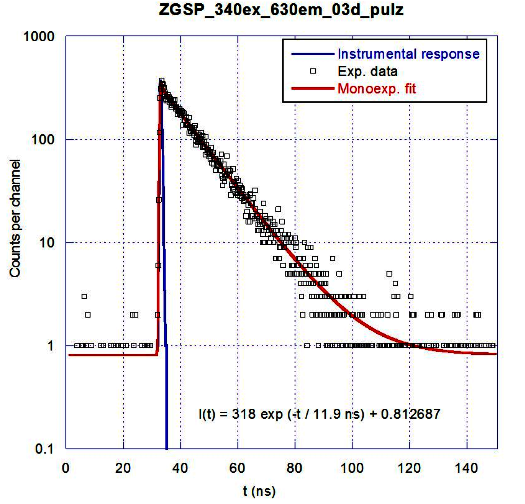
\includegraphics[width=0.6\textwidth]{pictures/zgsp_januar_340ex_630em.PNG}
        \caption{PL decay of {\znoo} in EtOH under \numprint[nm]{339} excitation, emission \numprint[nm]{630}.}
        \label{fig:zgsp_januar_340ex_630em}
    \end{figure}
    
    \begin{figure}
        \centering
        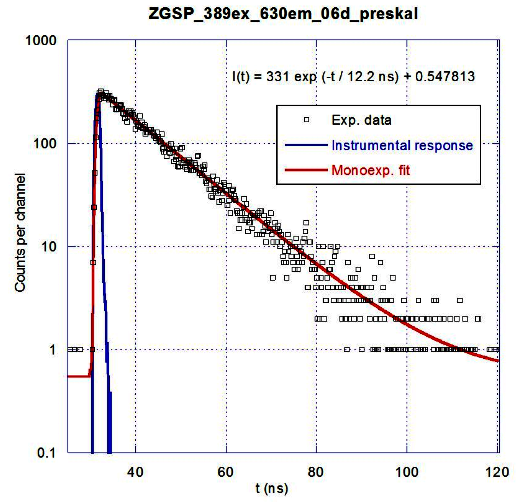
\includegraphics[width=0.6\textwidth]{pictures/zgsp_januar_389ex_630em.PNG}
        \caption{PL decay of {\znoo} in EtOH under \numprint[nm]{389} excitation, emission \numprint[nm]{630}.}
        \label{fig:zgsp_januar_389ex_630em}
    \end{figure}
    
    \subsection{Singlet oxygen production and detection}
    
    {\singlet} generation was investigated after X-ray irradiation of nanocomposite materials in solvent. The APF probe was used to indirect detection of {\singlet}. In short, absorption maximum of APF is at about \numprint[nm]{490} and oxidised form of APF is highly luminescent at \numprint[nm]{515}. Changes in luminescence of APF during irradiation were monitored. APF reacts with {\singlet} and with other ROS, moreover with -OH radicals \cite{bartosz06, setsukinai03}. Sodium azide {\azid} was chosen to distinguish emission which belongs to {\singlet} oxidation and emission which belongs to other ROS oxidisation. {\azid} is specific quencher of {\singlet} \cite{bulin13}. According to research in literature, concentration \numprint[mM]{10} of {\azid} in EtOH was used \cite{price09,bancirova11, huang12, liyi12}.
    
    After biofunctionalization the product consisted of dark coloured and light coloured part. The \cref{fig:xrd_zgsp_dark_fair} shows XRDP diffraction patterns for these two parts and silica coated precursor. It seems that both parts consist of nanoparticles ZnO:Ga. From the \cref{fig:xrdp_znO} it is obvious that diffraction patterns did not change during biofunctionalization. The XRDP pattern for dark coloured part of ZnO:Ga@SiO$_{2}$-PPIX indicates the samples contained a lot of amorphous phase, probably unbounded free PPIX.

        \begin{figure}
        \centering
        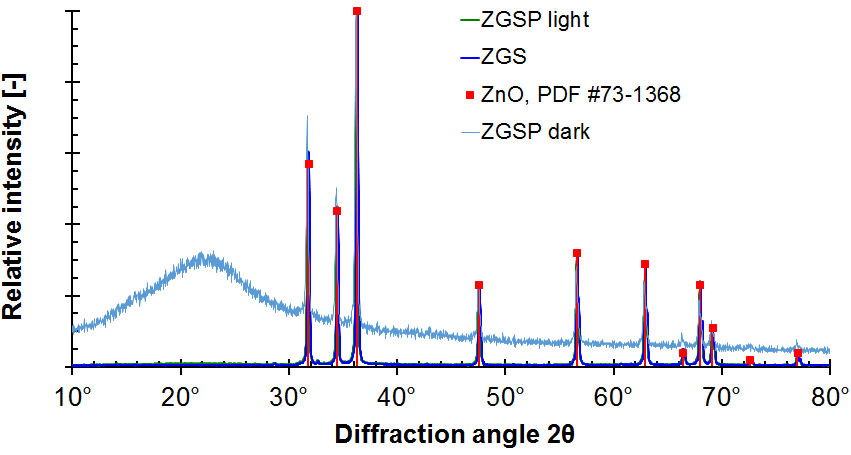
\includegraphics[width=0.6\textwidth]{pictures/xrd_zgsp_dark_fair.PNG}
        \caption{XRDP diffraction patterns for ZnO:Ga@SiO$_{2}$ (ZGS), light coloured part of ZnO:Ga@SiO$_{2}$-PPIX (ZGSP) and dark coloured part of ZnO:Ga@SiO$_{2}$-PPIX (ZGSP dark).}
        \label{fig:xrd_zgsp_dark_fair}
        \end{figure}
    
    The \cref{fig:apf_zgsp_dark_new_holder} shows spectra which belong to the dark coloured part of ZnO:Ga@SiO$_{2}$-PPIX. It is obvious that luminescence intensity decreases in time at peaks \numprint[nm]{590} and \numprint[nm]{650}. No luminescence increase is observed at maximum of APF at \numprint[nm]{520} as shown in the \cref{fig:apf_zgsp_dark_vyrez_new_holder}. The characterization of dark coloured part of ZnO:Ga@SiO$_{2}$-PPIX showed a small amount of ZnO:Ga in the sample, therefore the generation of {\singlet} could have been unmeasurable.

    The \cref{fig:apf_zgsp_fair_new_holder} shows spectra which belong to the light coloured part of ZnO:Ga@SiO$_{2}$-PPIX. Against the \cref{fig:apf_zgsp_dark_new_holder} luminescence intensity increases in time. The \cref{fig:apf_zgsp_fair_vyrez_new_holder} shows changes in APF luminescence in time. Unexpectedly, luminescence at peak \numprint[nm]{640} rises also as shown in the \cref{fig:apf_zgsp_fair_new_holder}. Previous experiments confirm that this peak belongs to PPIX and not to APF. Luminescence at peak \numprint[nm]{640} decreases  in the \cref{fig:apf_zgsp_dark_new_holder} unlike the increase in the \cref{fig:apf_zgsp_fair_new_holder}. The reduction could be caused by sedimentation of the nanocomposite material. We could not explain this luminescence rise in detail. Since measurements with {\azid} were not carried out within these samples we could not prove {\singlet} generation. However, the luminescence increase in the \cref{fig:apf_zgsp_fair_vyrez_new_holder} denotes {\singlet} production in time.

    \begin{figure}
        \centering
        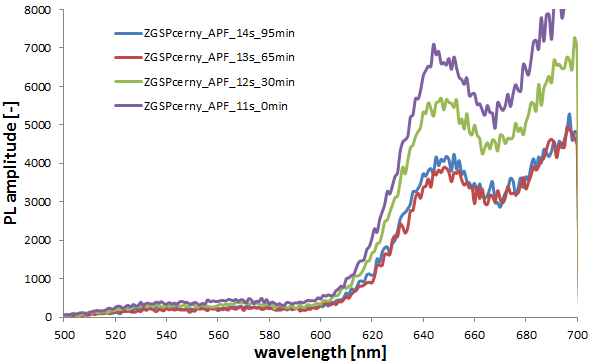
\includegraphics[width=0.6\textwidth]{pictures/apf_zgsp_dark_new_holder.PNG}
        \caption{PL emission spectra of dark coloured part of ZnO:Ga@SiO$_{2}$-PPIX (ZGSP) in EtOH under \numprint[nm]{470} excitation.}
        \label{fig:apf_zgsp_dark_new_holder}
    \end{figure}
    
    \begin{figure}
        \centering
        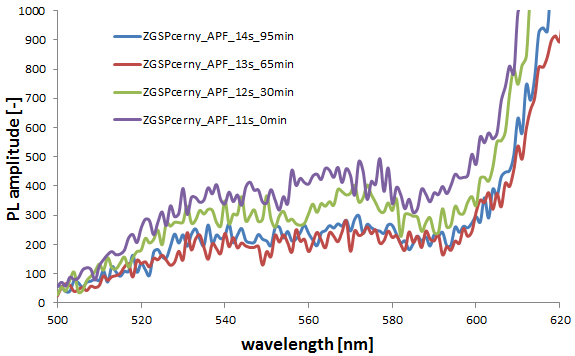
\includegraphics[width=0.6\textwidth]{pictures/apf_zgsp_dark_vyrez_new_holder.PNG}
        \caption{PL emission spectra of dark coloured part of ZnO:Ga@SiO$_{2}$-PPIX in EtOH under \numprint[nm]{470} excitation, monitoring APF.}
        \label{fig:apf_zgsp_dark_vyrez_new_holder}
    \end{figure}
    
    \begin{figure}
        \centering
        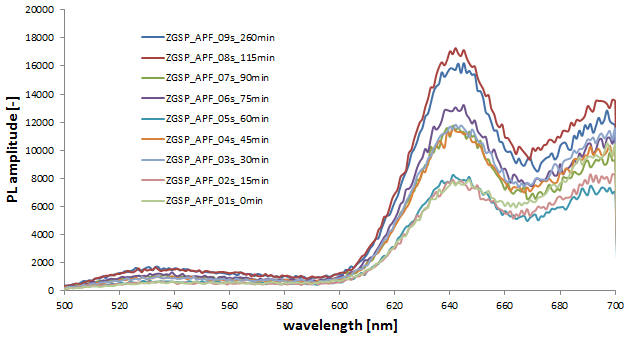
\includegraphics[width=0.6\textwidth]{pictures/apf_zgsp_fair_new_holder.PNG}
        \caption{PL emission spectra of light coloured part of ZnO:Ga@SiO$_{2}$-PPIX (ZGSP) in EtOH under \numprint[nm]{470} excitation.}
        \label{fig:apf_zgsp_fair_new_holder}
    \end{figure}
    
    \begin{figure}
        \centering
        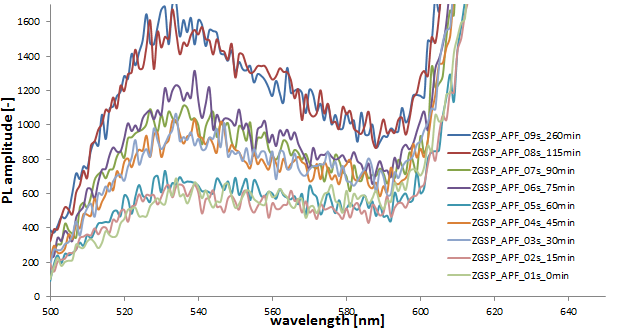
\includegraphics[width=0.6\textwidth]{pictures/apf_zgsp_fair_vyrez_new_holder.PNG}
        \caption{PL emission spectra of light coloured part of ZnO:Ga@SiO$_{2}$-PPIX in EtOH under \numprint[nm]{470} excitation, monitoring of APF.}
        \label{fig:apf_zgsp_fair_vyrez_new_holder}
    \end{figure}
    